
\documentclass{article}
\usepackage{lmodern}
\usepackage[T1]{fontenc}
\usepackage{shapepar}
\usepackage{microtype}
\usepackage{lipsum}
\usepackage{pgfplots}
\pgfplotsset{compat=1.9}
\usepackage{tikz}
\usetikzlibrary{calc,fit,intersections,folding}
\usepackage{pstricks-add}
\usetikzlibrary{arrows.meta,angles,arrows,quotes,backgrounds,calc}
\usepackage[left = 5mm, right = 5mm, top = 5mm, bottom = 5mm]{geometry}



\setlength{\parindent}{0em}

\newcommand{\clrone}{blue}
\newcommand{\clrtwo}{red}

\begin{document}
\thispagestyle{empty}

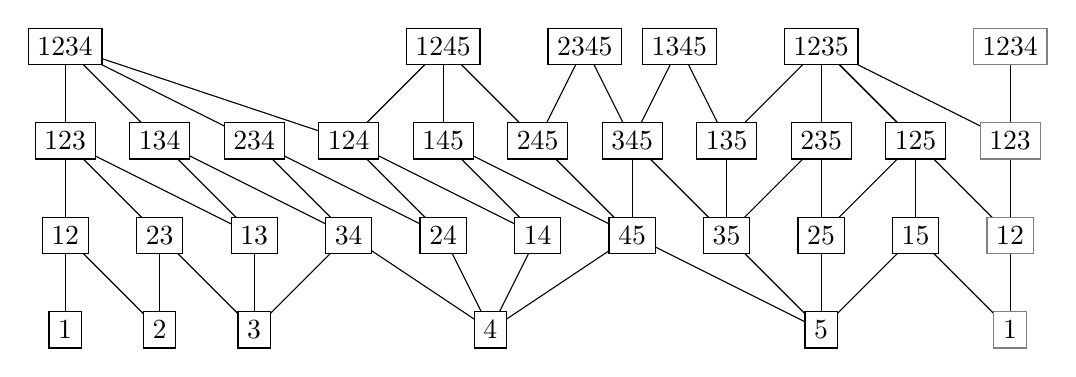
\begin{tikzpicture}[scale = 0.6]
\coordinate (12) at (0, 2);
\coordinate (23) at (2,2);
\coordinate (13) at (4,2);
\coordinate (34) at (6,2);
\coordinate (24) at (8,2);
\coordinate (14) at (10,2);
\coordinate (45) at (12,2);
\coordinate (35) at (14,2);
\coordinate (25) at (16,2);
\coordinate (15) at (18,2);
\coordinate (12e) at (20,2);

\coordinate (1) at (0,0);
\coordinate (2) at (2,0);
\coordinate (3) at (4,0);
\coordinate (4) at (9,0);
\coordinate (5) at (16,0);
\coordinate (1e) at (20,0);

\coordinate (123) at (0,4);
\coordinate (134) at (2,4);
\coordinate (234) at (4,4);
\coordinate (124) at (6,4);
\coordinate (145) at (8,4);
\coordinate (245) at (10,4);
\coordinate (345) at (12,4);
\coordinate (135) at (14,4);
\coordinate (235) at (16,4);
\coordinate (125) at (18,4);
\coordinate (123e) at (20,4);

\coordinate (1234) at (0,6);
\coordinate (1245) at (8,6);
\coordinate (2345) at (11,6);
\coordinate (1345) at (13,6);
\coordinate (1235) at (16,6);
\coordinate (1234e) at (20,6);



\foreach \a/\b in {1/12,2/12,2/23,3/23,3/13,3/34,4/34,4/24,4/14,4/45,5/45,5/35,5/25,5/15,12/123,23/123,13/123,13/134,34/134,34/234,24/234,24/124,14/124,45/145,45/245,45/345,35/345,35/135,35/235,25/125,15/125,123/1234,134/1234,234/1234,124/1234,124/1245,145/1245,245/1245,245/2345,345/2345,345/1345,135/1345,135/1235,235/1235,125/1235, 14/145,125/1235,12e/125, 123e/1235, 1e/15,1e/12e,12e/123e,123e/1234e,25/235}
{  \draw (\a) -- (\b);  }


\foreach\n in {1,2,3,4,5,12,13,14,15,23,24,25,34,35,45,123,124,125,134,135,145,234,235,245,345,1234,1235,1345,1245,2345}
{ \node[draw, fill = white] at (\n) {$\n$}; }

\node[draw=gray, fill=white] at (1e) {$1$};
\node[draw=gray, fill=white] at (12e) {$12$};
\node[draw=gray, fill=white] at (123e) {$123$};
\node[draw=gray, fill=white] at (1234e) {$1234$};

\end{tikzpicture}

\end{document}